\documentclass[dissertation.tex]{subfiles}
\begin{document}

\chapter[Identifying Optimal Biomarkers for Clinical Tests][Finding Optimal Biomarkers]{Identifying Optimal Biomarkers for Clinical Tests}
\label{chap:messina}


\emph{Thesis: Decision stump classifiers can be efficiently trained on high-throughput biomarker data, and provide a principled way to translate large multi-measurement research data into simple but high-performance clinical tests.}


\paragraph{Summary}


\section{Introduction}

Research and molecular pathology laboratories take strikingly different approaches to the measurement of biomarkers in patient samples.  Research work favours costly manual techniques, which quantify a large number of biomarkers in a relatively small number of samples.  Conversely, pathology laboratories make extensive use of highly automated turnkey systems, to robustly measure a relatively small number of biomarkers in a large number of samples.  In keeping with this divide, research and pathology laboratories often use very different technologies for the measurement of the same type of biomarker, such as RNA sequencing in research, and quantitative PCR in the clinical realm.  This difference in base technology, and the generally increased variability of clinical samples over research ones~\cite{Hewitt2008}, complicates the translation of discoveries in research into application in the clinic.

Although difficult, this translation of research discoveries into clinical practice is absolutely necessary.  Research and pathology techniques are complementary: biomarker discovery requires research techniques capable of interrogating a huge number of potential biomarkers, but the \emph{application} of any discoveries must use pathology techniques that can reliably and economically handle a potentially huge number of patient samples.  Finding effective ways to translate research findings into clinical application is critically important.  This problem can be approached from two angles: by harmonising measurement technology between research and diagnostic laboratories, or by identifying lead biomarkers in the research laboratory that have a high likelihood of effectively translating to diagnostic measurement.  The former approach may represent a long-term solution, but does not reflect the current state of technology.  To implement the latter approach requires bioinformatic techniques that can search large bodies of research measurement data, to identify a small number of biomarkers that are most likely to make good diagnostic tests.

Effective clinical tests must satisfy a number of requirements, which can be used to guide the translation of a research finding into a clinical tool.  Ideally, a clinical diagnostic or prognostic test should be based on the measurement of only a small number of biomarkers~\cite{Lesko2001, Pepe2001}.  Additionally, it should be highly robust to technical effects, and the inevitable variation in sample quality and handling that comes with clinical specimens~\cite{Hewitt2008}.  The results of most tests will be interpreted as a simple binary variable\footnote{For example, disease versus not diseased, responder versus non-responder, or poor prognosis versus good prognosis.}, and the detection performance of this binary variable should match the particular clinical application~\cite{Pepe2001}.  Taking all these requirements into account, a technique to translate discovery biomarker measurements into a clinical test should be able to process measurements of thousands of biomarkers to identify those single biomarkers that, when their level is thresholded, yield a particular class separation performance, with maximal robustness to technical effects.

Existing methods for the mining of research data for potential biomarkers do not meet these requirements.  For both diagnostic and prognostic endpoints, common biomarker prioritization techniques either do not provide fine control of classification accuracy and robustness, or yield sets of biomarkers that are far too large to practically deploy.  Two broad strategies are generally employed to identify biomarkers in large research data sets: univariate statistics, and machine learning.  The first strategy encompasses approaches such as per-biomarker regression tests for association between the biomarker and a sample group or outcome, and the second covers the use of algorithms such as \glspl{SVM} to construct high-performance predictors of group or prognosis from the measurements of many biomarkers.

Univariate statistic approaches identify single biomarkers of interest, but supply no guarantee as to the suitability of these biomarkers for translation into clinical tests.  These statistics are designed to identify differences in average value between two groups, not to construct classifiers.  Significance testing and classifier learning are distinct problems, and usually have different solutions: a biomarker that shows a statistically significant difference in signal between two groups may still be a poor classifier; and vice versa (\fref{fig:messina-example-stats-class}).  Univariate tests also do not take the particular requirements of a clinical problem into account.  For example, consider two tests for the same disease -- one test is intended to be used as a population screen, and the other to rule out a suspected diagnosis.  These two tests would have very different performance requirements, and quite possibly would be best served by two different biomarkers.  Univariate test approaches to candidate biomarker selection cannot take this nuance into account, which further limits their usefulness for biomarker selection.
% These special test performance requirements can be accommodated by machine learning algorithms, but the classifiers produced by these algorithms are also usually poorly-suited to clinical test development.
% Mention that this is because of the sqrt(n) factor in the tests?  Testing hypotheses on population mean, not on population distrib.

\begin{figure}[!htbp]
  \centering
  \vspace{1cm}
  \subbottom[Poor classification]{
    \def\svgwidth{.4\linewidth}
	\input{messina_class_test_comparison_a.pdf_tex}
    \label{fig:messina-example-stats-class-stat}}
  \hspace{1cm}
  \subbottom[Good classification]{
    \def\svgwidth{.4\linewidth}
	\input{messina_class_test_comparison_b.pdf_tex}
    \label{fig:messina-example-stats-class-class}}
  \caption[Statistical significance does not imply good classification ability]{Statistical significance does not imply good classification ability.  The left and right panels show the distributions of two hypothetical biomarkers, $a$ and $b$, in two sample classes, shown in orange and green.  The intent is to construct a single-feature classifier separating the two sample classes.  The levels of biomarker $a$ (left panel) are significantly different between the two classes, but the large overlap in distributions would make it a poor choice for a classifier, with sensitivity and specificity both approximately $0.6$.  Conversely, biomarker $b$ (right panel) could be used to form an effective threshold-based classifier, with sensitivity and specificity each around $0.8$.  This comparison also demonstrates the unsuitability of many univariate statistical tests for classifier selection: for example, biomarker b does not show significantly different expression between the groups by the t and Mann-Whitney U tests, although it does by the more general Kolmogorov- Smirnov test (data not shown).}
\label{fig:messina-example-stats-class}
\end{figure}

Machine learning algorithms can produce highly accurate classifiers matching given performance requirements~\cite{Bach2006}, but these classifiers generally rely on combining information from a large number of biomarkers.  This has not entirely prevented multi-gene tests based on these classifiers from achieving clinical use (an early example of a multi-gene clinical test is MammaPrint\texttrademark, a simple linear classifier based on measurements of 70 transcripts~\cite{Veer2002}), but does drastically increase the complexity of translation from the research laboratory to the clinical, and the final cost of the test (for MammaPrint, approximately \fcardinal{4200} USD per patient).  As well as being difficult to translate into a clinical diagnostic, high-performance multi-feature classifiers require care when training~\cite{Aliferis2009}, their complex workings usually defy human interpretation~\cite{Breiman2001b}, and their complexity often simply isn't required for good classification~\cite{Grate2005}.  Many approaches are available to limit the number of biomarkers in classifiers returned by machine learning algorithms~\cite{Guyon2003}, but as the number of biomarkers is reduced to one, this generally comes at the cost of performance (TODO cite?).  For the limiting case of single-biomarker classifiers and prognostics, a machine learning algorithm designed exclusively for the task is needed.

To address this need, in 2009 I reported the Messina algorithm, for the efficient cost-sensitive training of single-feature binary threshold classifiers~\cite{Pinese2009}.  The single-feature binary threshold classifiers found by Messina use the abundance of a single biomarker to place samples into two groups: one containing samples with biomarker levels below a threshold, and the other containing samples with biomarker levels at or above the threshold.  Given measurements of many biomarkers in a set of samples from two groups, Messina identifies the biomarkers, and their optimal thresholds, that will separate the two groups well.  Messina could be used to address two problems: the selection of biomarkers that are well-suited for development into single-measurement diagnostic tests, and the identification of biomarkers with differential signal between two sample groups.  The latter functionality was the focus of the original Messina paper, which demonstrated that Messina was a strong alternative to more classical tests of differential expression, that allowed the user to smoothly trade robustness to outliers against sensitivity to subtle changes in expression.  Messina was recommended by an independent comparison of outlier differential expression methods~\cite{Karrila2011}, but remains a relatively limited tool: Messina is only available as a standalone program, and its objective function is hard-coded for binary classification, and so it can not generate more general classifiers, such as for prognosis.

Tools to identify biomarkers that can yield accurate estimates of prognosis remain relatively crude, compared to those for classification problems.  As discussed in \Cref{chap:nomogram}, there is a pressing need in \gls{PDAC} for effective methods to preoperatively stage patients.  Biomarkers of prognosis can be measured preoperatively, but the S100A2 and S100A4 markers tested in \Cref{chap:nomogram} were relatively poor at predicting outcome following resection of \gls{PDAC}.  S100A2 and S100A4 were identified following only a small candidate screen, and it is reasonable to expect that a global search for \gls{PDAC} biomarkers of prognosis will yield candidates with better performance.  Prognostic tests have the same clinical translation requirements as diagnostic tests: they must be based on a small number of biomarker measurements, and by simple thresholding of these measurements, yield a robust prediction of differential outcome.  Machine learning algorithms such as random forests and \glspl{SVM} have been adapted to the prediction of outcome, but suffer the same general problem of machine learning solutions: too many biomarkers must be measured to achieve accurate prediction.  Most univariate statistics approaches also suffer the same problem as their classification counterparts, by failing to take the particular class separation needs of the application into account.  These problems with conventional approaches have led to the common use of ad-hoc analyses when identifying biomarkers of prognosis.

The poor suitability of conventional approaches for identifying biomarkers of prognosis has led to the common use of ad-hoc analyses for this problem, but these usually perform very poorly.  Methods in common use are the median cut, in which the cohort is divided into two groups by the median value of each biomarker, and then a log-rank test performed on these two groups; and the so-called `optimal' cut, in which many cutpoints are tried, and the best log-rank statistic is used as the final test statistic.  The median cut approach presupposes that the poor- and good-prognosis subgroups in the data are equal in size, and has poor power if this is not the case, and the `optimal' cut procedure is decidedly non-optimal, with an unsurprising high false detection rate due to uncorrected multiple testing.  Although discussion of the significant deficiencies in these approaches has been in the medical literature for over twenty years~\cite{Altman1994}, they continue to see routine use and further development~\cite{Budczies2012,Camp2004,Chorlton2014,Yau2010}.  A natural approach to correcting the `optimal' procedure is by incorporating multiple testing correction, and software is available to perform this as \texttt{R} package \texttt{maxstat}~\cite{Chorlton2014,Hothorn2003}.  However, in common with more conventional univariate approaches, \texttt{maxstat} and similar methods do not allow for control over any desired aspects of the prognostic classifier, such as the hazard ratio between the poor- and good-prognosis groups, or the relative group sizes.  As in the classification case, a biomarker selection procedure specifically designed for clinical translation is needed.

In this chapter I present Messina2, a general algorithm for single-feature threshold classifier learning.  Like its predecessor Messina, Messina2 aims to produce maximally robust classifiers that satisfy user-supplied performance requirements.  Unlike Messina, Messina2 accepts any performance metric, and so can be used to create binary classifiers for any task, including diagnosis and prognosis.  Messina2's emphasis on maximally robust classifiers means that the biomarkers that it selects are especially well suited for translation to the clinical diagnostic laboratory, helping to address the divide between research discovery and clinical application.  To facilitate Messina2's use in bioinformatic workflows, it has been made into the \texttt{R} package \texttt{messina}, available as part of the Bioconductor project~\cite{Gentleman2004}\footnote{The version of Messina2 used for this thesis is not yet in the latest Bioconductor release.  To access the thesis version, clone the \texttt{thesis} branch from the Bitbucket repository \texttt{marpin/r-messina}, or from \texttt{R}, with \texttt{devtools} installed, run the command \texttt{ devtools::install\_bitbucket("marpin/r-messina", ref = "thesis")}.}.  This chapter will describe the general framework of binary threshold classifiers, detail the Messina2 algorithm and how it differs from Messina, and demonstrate its characteristics and performance relative to other techniques.  An application to the problem of identifying better prognostic biomarkers in pancreas cancer will illustrate the utility of Messina2 in real data.

\section{Messina and Messina2}
Messina and Messina2 are algorithms that take as input measurements of biomarker abundance in a number of samples, and return as output threshold classifiers that can separate the input samples into two groups.  For Messina, these groups are based on user-supplied sample labels, such as cancer and non-cancer, and the classifiers are designed to separate these two sample types as robustly as possible, whilst still meeting user-supplied minimum sensitivity and specificity requirements\footnote{Here sensitivity and specificity are used in their binary classification sense.  In a binary classification problem (for example, a diagnostic test to detect the presence of a disease, where the result is either `diseased,' or `not diseased,' with no intermediate `uncertain'), a given classifier tested on a population of samples will have associated rates of true positive, true negative, false positive, and false negative calls.  The sensitivity of this classifier on that population is then the true positive call rate divided by the total positive sample rate, and the specificity is the true negative call rate divided by the total negative sample rate.  Symbolically, let $R_{ab}$ be the rate at which a sample which is truly of class $a$ is called as class $b$, $a, b \in \{0,1\}$, where $1$ represents the positive class, and $0$ the negative.  Then, $\mathrm{Sens} = p_n = R_{11} \div R_{1\bullet}$, and $\mathrm{Spec} = p_c = R_{00} \div R_{0\bullet}$.}.  Messina2 is more general, and can produce both diagnostic and prognostic classifiers, by identifying thresholds that satisfy any user-supplied objective function.  As the Messina2 algorithm is both more general than, and very similar to, Messina, this chapter will primarily describe Messina2, drawing comparisons to Messina where appropriate.

\subsection{Algorithm}
Messina2 operates on each biomarker in a data set separately, reporting whether that biomarker can be used to build a threshold classifier with the desired performance characteristics, and, if so, the optimal such classifier.  We represent the available data for a given biomarker as pairs of the form $(x_i, y_i)$, where $x_i \in \mathbb{R}$ is the biomarker abundance, and $y_i \in \mathbb{Y}$ is a dependent variable that we wish to predict in new samples, for sample $i$ of $n$ samples total.  The domain of $y_i$, $\mathbb{Y}$, depends on the problem at hand, and is determined by the form of the objective function\footnote{For example, in classification, $y_i \in \{0, 1\}$, whereas for right-censored survival analysis, $y_i$ is a (time, event) pair, $y_i \in (\mathbb{R}^+, \mathbb{B})$.}.

The core Messina2 learning process is given in Algorithm \ref{alg:mess-messina2}.  

\begin{algorithm}[!htbp]
  \KwData{An $n$-tuple of covariate measurements $x$, an $n$-tuple of associated dependent values $y$, a minimum subclass fraction $b$, and an objective function $f: (\mathbb{B}^n, \mathbb{Y}^n) \rightarrow \mathbb{B}$.  $x$ and $c$ are to be in ascending order.  The domain of $y$ is given as $\mathbb{Y}^n$, as it varies between modes of Messina.}
  \KwResult{A tuple of three values.  If the fit failed, $(0, 0, 0)$.  If the fit succeeded, (optimal classifier threshold, optimal classifier direction, resultant classifier margin).}

  \Begin {
  	\tcp{Define candidate thresholds $c$ as the midpoints between consecutive unique values of $x$}
  	$c \longleftarrow \mathrm{MakeCutpoints}\left(x, b\right)$\;
  	$m \longleftarrow \vert c \vert$\;
  
	\tcp{Test the objective $f$ on each threshold in $c$}
	\For{$i \leftarrow 1$ \KwTo $m$}{
		$w^+ \longleftarrow \left(~\left[x_j \geq c_i\right]~\right)_{j=1}^n$\;
		$w^- \longleftarrow \left(~\left[x_j < c_i\right]~\right)_{j=1}^n$\;
		$o^+_i \longleftarrow f\left(w^+, y\right)$\;
		$o^-_i \longleftarrow f\left(w^-, y\right)$\;
	}
	
	\tcp{If no threshold passed $f$, return $\varnothing$}
	\If{$o^+ \vee o^-$ is all $\mathrm{false}$}{
      \KwRet $\varnothing$\;
    }
	
	\tcp{Search $o^+$ and $o^-$ for the widest margin contiguous interval that passes $f$}
	$(t^+, \Delta^+) \longleftarrow$ BestInterval$\left(o^+, c\right)$\;
	$(t^-, \Delta^-) \longleftarrow$ BestInterval$\left(o^-, c\right)$\;
	
	\tcp{Return the best of the $o^+$ and $o^-$ results}
	\eIf{$\Delta^+ \geq \Delta^-$}{
	  \KwRet{$(t^+, +1, \Delta^+)$}\;
	}{
	  \KwRet{$(t^-, -1, \Delta^-)$}\;
	}
  }
  \caption[MessinaCore]{MessinaCore.  Searches the real line for the largest interval for which the objective $f(w, y)$ is true, and returns the centre and half-width of that interval.}
  \label{alg:mess-core}
\end{algorithm}

The user-specified objective function $f(w, y)$, $f: (\mathbb{B}^n, \mathbb{Y}^n) \rightarrow \mathbb{B}$ is the core of the Messina2 algorithm.  It takes as input $w$, a binary $n$-vector that separates the samples into two groups, and the dependent variable $y$, and returns $\mathrm{true}$ if the data split given by $w$ provides a desired separation of the values of $y$, or otherwise $\mathrm{false}$.  The data split $w$ is made by testing the values of $x$ against a threshold $t \in \mathbb{R}$, as $w_i = [x_i \geq t]$; $f(w, y)$ therefore tests whether cutting the samples into two groups, one with $x < t$, and the other with $x \geq t$, yields a desired difference in $y$ between the two groups.  The form of $f$ is completely under user control, although the Messina2 package does provide some reasonable defaults that yield classifiers with certain desirable characteristics.

In all practical cases, either $f(w, y) = \mathrm{false}$ for all $t$, or there will be a range of thresholds $t$ for which $f(w, y) = \mathrm{true}$.  In the former case, the biomarker under consideration is discarded by Messina2, but in the latter case, a principled way is needed to choose an optimal threshold $t^* \in \{t~:~t \wedge f(w, y) = \mathrm{true}\}$.  For this task, Messina2 uses a maximum margin heuristic and chooses $t^*$ as the midpoint of the largest real interval for which $f(w, y) = \mathrm{true}$.  The intuition behind this selection is that such a choice of threshold maximises the size of the smallest threshold perturbation that is necessary to make the classifier violate its performance requirements, that is, 
\begin{equation}
t^* = \argmax_t \mathrm{min}\{ \vert\delta\vert~:~\delta \in \mathbb{R} \wedge \neg f\left(~\left(~[x_i \geq t + \delta]~\right)_{i=1}^n, y\right) \}
\end{equation}
where $f([~[x_i \geq t + \delta]~]_{i=1}^n, y)$ is the value of the objective $f$ when the threshold $t + \delta$ is applied to the data $x$, with $\delta$ the perturbation.

Messina2 considers all possible thresholds $t \in \mathbb{R}$ when searching for the optimal threshold $t^*$, and as such is at risk of overfitting the data, and reporting spurious classifiers.  To overcome this problem, Messina2 by default employs an outer bootstrap loop to verify that a classifier under consideration still satisfies the objective function $f$, when tested on holdout data.  Multiple bootstrap draws of the data $(x, y)$ are made, and for each draw a Messina2 classifier is trained on the drawn samples, the trained classifier is used to separate the undrawn (so-called `out-of-bag') samples into two classes, and the objective $f$ is evaluated on the resulting separation of the out-of-bag data.  Messina2 only returns classifiers for which the objective $f$ is $\mathrm{true}$ in at least half of the out-of-bag evaluations.  This outer bootstrap layer adds an additional level of stringency to the Messina2 results, but dramatically increases the runtime of the algorithm, and in some applications may not be required: the Vapnik–Chervonenkis dimension of a single-feature threshold classifier is $2$, and so Messina2's potential for overfitting is relatively low~\cite{Vapnik1999}, even before bootstrapping is performed.

\subsection{Objective functions}
Messina2 is designed to accept any objective function $f$, to allow custom analyses, but is also supplied with two reasonable default objective functions, designed to handle common tasks in classification and survival analysis.

The objective function $f_M$ is designed to mimic the behaviour of the original Messina algorithm for classification and differential expression detection.  This function returns $\mathrm{true}$ if the data split $w$ separates the classes in $y$, with sensitivity and specificity at least as good as user-supplied minimum values:
\begin{align*}
f_M(w, y) &= \left[ p_n \geq l_n \wedge p_c \geq l_c \right] \\
p_n &= \frac{\sum_i{\left[ w_i \wedge y_i \right]}}{\sum_i{\left[ y_i \right]}} \\
p_c &= \frac{\sum_i{\left[ \neg w_i \wedge \neg y_i \right]}}{\sum_i{\left[ \neg y_i \right]}} \\
\end{align*}
In the above, $p_n$ and $p_c$ are the observed sensitivity and specificity, respectively, and $l_n$ and $l_c$ are their user-supplied minimum acceptable values.  When used with this objective function, Messina2 will return maximum-margin classifiers that separate the two groups defined in $y$ with at least the required minimum sensitivity and specificity.  When identifying lead biomarkers for the construction of a clinical test, the analyst can set the sensitivity and specificity requirements to values matching the intended application of the test, and be confident that the biomarkers reported by Messina2 will robustly separate the sample groups with at least this desired level of performance.

TODO: ADVANTAGE OVER ROC.  See above para.  So basically, someone might argue -- why not just do a ROC with a cost-sensitive threshold?  That way it can be done with any classifier that gives a continuous output.  Problem is that the ROC doesn't include margin information.  So it's not just about hitting the right balance of sens & spec, but doing so ROBUSTLY.  How sure can we be that our target sens & spec will be achieved on a test set?  What about a completely different cohort?  Using a different technology?  Best option is to MAXIMIZE MARGIN.  I need to put this thinking somewhere.

The objective function $f_H$ is intended for survival analysis, where the goal is to identify biomarkers that can robustly separate a cohort into good- and poor-outcome groups.  Messina2 in this mode provides a more principled approach to thresholding biomarker levels for prognosis than the commonly employed median-cut or multiple-cut procedures \cite{TODO}.  $f_H(w, y)$ returns $\mathrm{true}$ if the approximate hazard ratio (using survival data in $y$) between the groups defined by $w$ is at least a user-supplied value.  The approximate hazard ratio is calculated from the log-rank test statistic, as:
\begin{align*}
f_H(s, y) &= \left[ \vert \log{p_h} \vert \geq \log{l_h} \right] \\
\log{p_h} &= Z\sqrt{\frac{4}{n_e}}
\end{align*}
where $p_h$ is the approximate hazard ratio achieved by the data split in $w$, $l_h$ is the minimum hazard ratio desired, $Z$ is the value of the log-rank test statistic\footnote{$Z$ is the signed log-rank test statistic, not to be confused with the $\Chi^2$ statistic, which is also used.  $\Chi^2 = Z^2$.}, and $n_e$ is the number of events in $y$.

\subsection{Algorithm}
\begin{algorithm}
  \KwData{An $n$-tuple of covariate measurements $x$, an $n$-tuple of associated dependent values $y$, an objective function $f: (\mathbb{B}^n, \mathbb{Y}^n) \rightarrow \mathbb{B}$, a minimum subclass fraction $b$, and a number of bootstrap rounds $r$.  $x$ is to be sorted in ascending order.  The domain of $y$ is given as $\mathbb{Y}^n$, as it varies between modes of Messina.}
  \KwResult{If the fit failed, $\varnothing$.  Otherwise, a tuple of two real values: $(t^*$, $\Delta^*)$, encoding the optimal classifier threshold, resultant classifier margin).}

  \Begin {
  	$n_{\mathrm{pass}} \longleftarrow 0$\;
  	\For{$i \leftarrow 1$ \KwTo $r$}{
  		\tcp{Generate a bootstrap sample of (x, y)}
  		$(x_{\mathrm{in}}, y_{\mathrm{in}}, x_{\mathrm{out}}, y_{\mathrm{out}}) \longleftarrow \mathrm{BootstrapSample}\left( x, y \right)$\;
  		
  		\tcp{Train MessinaCore on this bootstrap sample}
  		$(t_{\mathrm{in}}, d_{\mathrm{in}}, \Delta_{\mathrm{in}}) \longleftarrow \mathrm{MessinaCore}\left( x_{\mathrm{in}}, y_{\mathrm{in}}, b, f \right)$\;
  		
  		\tcp{Assess performance of the MessinaCore classifier on the out-of-bag samples}
  		\If{$d_{\mathrm{in}} \neq 0$}{
  			$w_\mathrm{out} \longleftarrow \left(~\left[ x_{\mathrm{out}_j} d_{\mathrm{in}} \geq t_{\mathrm{in}} d_{\mathrm{in}}\right]~\right)_{j=1}^{\vert x_\mathrm{out} \vert}$\;
  			\If {$f\left(w_\mathrm{out}, y_{\mathrm{out}}\right) = \mathrm{true}$}{
  				$n_{\mathrm{pass}} \longleftarrow n_{\mathrm{pass}} + 1$\;
  			}
  		}
  	}
  	
  	\tcp{Did the in-bag trained classifiers satisfy out-of-bag performance requirements in at least half of the bootstrap rounds?}
  	\eIf{$r = 0 \vee n_{\mathrm{pass}} \geq \frac{1}{2}r$}{
	  	\tcp{Yes; return the fit on the full data}
  		\KwRet{$\mathrm{MessinaCore}\left( x, y, b, f \right)$}\;
  	}{
  		\tcp{No; this fit failed.}
  		\KwRet{$\varnothing$}\;
	}
  }
  \caption[Messina2]{Messina2.  This is essentially a bootstrap validation wrapper around MessinaCore, which in turn performs the core learning.  The purpose of the wrapper is to ensure that the MessinaCore classifiers satisfy the objective function, when assessed on out-of-bag data.  $\mathrm{BootstrapSample}$ is a function that generates a bootstrap sample of its matched tuple arguments $x$ and $y$, returning both the in-bag and out-of-bag $x$ and $y$ values as tuples.  If the number of bootstrap iterations $r$ is zero, no bootstrap validation is performed and this algorithm effectively falls through to MessinaCore.}
  \label{alg:mess-messina2}
\end{algorithm}

\begin{algorithm}
  \KwData{$o \in \mathbb{B}^m$, $c \in \mathbb{R}^m$, $x \in \mathbb{R}^n$}
  \KwResult{$(t^* \in \mathbb{R}, \Delta^* \in \mathbb{R}^+)$}

  \Begin {
    $\Delta^* \longleftarrow 0$\;
    $t^* \longleftarrow 0$\;
    
    $i \longleftarrow 1$\;
    \While{$i \leq m$}{
      \If{$o_i$ is $\mathrm{true}$}{
        $r_L \longleftarrow \sup \{x_k~|~x_k \leq c_i \wedge k \in \mathbb{N}^+ \wedge k \leq n \}$\;
        \For{$j \leftarrow i$ \KwTo $m$}{
          \eIf{$o_j$ is $\mathrm{true}$}{
            $r_R \longleftarrow \sup \{x_k~|~x_k \leq c_j \wedge k \in \mathbb{N}^+ \wedge k \leq n \}$\;
          }{
            break\;
          }
        }

		$\Delta \longleftarrow \frac{1}{2}\left(r_R - r_L\right)$\;
        \If{$\Delta > \Delta^*$}{
          $\Delta^* \longleftarrow \Delta$\;
          $t^* \longleftarrow r_L + \frac{1}{2}\Delta$\;
        }
        
        $i \longleftarrow j$\;
      }
      $i \longleftarrow i + 1$\;
    }
    \KwRet{$(t^*, \Delta^*)$}\;
  }
  
  \caption[BestInterval]{BestInterval.}
  \label{alg:mess-bestinterval}
\end{algorithm}

\begin{algorithm}
  \KwData{An $n$-tuple of covariate measurements $x$, and a minimum subclass fraction $b$.  $x$ is to be sorted in ascending order.}
  \KwResult{A tuple of candidate cutpoints $c$, with values sorted in ascending order.}

  \Begin {
  	$x' \longleftarrow \mathrm{unique}(x)$\;
  	\For{$i \leftarrow 1$ \KwTo $\vert x' \vert - 1$}{
  		$p \longleftarrow \frac{1}{2} \left({x'}_i + {x'}_{i+1}\right)$\;
  		$s \longleftarrow \frac{1}{n} \sum_{i=1}^n \left[ x_i < p \right] $\;
  		\If{$s \geq b \wedge s \leq 1-b$}{
	  		$c \longleftarrow c \oplus p$\;
	  	}
  	}
  	\If{$b = 0$}{
	  	$c \longleftarrow -\infty \oplus c \oplus \infty$\;
	}
  	
	\KwRet{$c$}\;
  }
  \caption[MakeCutpoints]{MakeCutpoints.  Returns a sorted list of candidate cutpoints, each dividing the values in $x$ into two groups, with the restriction that all groups must contain at least fraction $b$ of the original values of $x$.  The function $\mathrm{unique}$ accepts a tuple argument, and returns a tuple containing the unique values of its argument, in ascending order.}
  \label{alg:mess-cutpoints}
\end{algorithm}



\begin{figure}[!htbp]
\centering
\def\svgwidth{\linewidth} 
\input{messina_class_cdfs.pdf_tex}
\caption[]{}\label{fig:mess-class-cdf-link}
\end{figure}


\section{Results}


\subsection{Messina2 is more effective than maxstat at finding validating biomarkers}

\subsection{Application of Messina2 to identify biomarkers for \acrshort{PDAC} prognosis}

\section{Discussion}

\section{Methods}


\begin{verbatim}
"How can we select markers that have the best possible chances of making it in the clinic?"

* Ok, now chapter outline:
  1) Messina
  2) Messina2
  3) Simulation Experiments:
     A) Margin => Perf robustness.  Two expts: symbolic on class, simul on surv.
     B) Messina2 class better than competing approaches.
     C) Messina2 surv better than competing approaches.
  4) Application example: MessinaSurv on APGI to find better biomarker leads.
  5) Discussion
  6) Methods (for sims only -- cover algos in 1 \& 2)

The Messina chapter.  What is this all about?  Selecting biomolecules.  For what purpose?  Differently how?  What makes this special?

OK back up.  Let's go back to basics.  Consider this situation.  There is a need to develop a diagnostic or prognostic test, for clinical application.  What requirements does this test have?
  * High performance
    - But notably, performance can be nuanced, not simply correct -- perhaps some errors are preferable to others.
  * Robustness (ie. performance is good, even in the face of:
    - cohort differences
    - technical differences (eg inter-lab)
    - sample handling differences (eg degradation, alternate storage or processing, sample age)
  * Ease of use
    - measures a small number of variables, as small as possible.
  * Translatability (can be easily moved to a clinical setting)
    - measures a small number of variables
    - uses existing technologies, as much as possible

Rolling all these together, it means we basically need an IHC- or ELISA-based measurement, on as few biomarkers as possible.  Just one would be ideal.

So what do we know about IHC?
  * It's very nonlinear
  * It's protein level based
  * There can be significant differences between labs, due to tissue processing, AR, and staining.  The latter two are less serious for clinical-grade stuff, but tissue processing is still a problem.  Time before fixation, conditions before fixation, time in fixative, type of fixative, conditions of embedding, time in storage in paraffin.
  * There can be differences between pathologists re: scoring.

What we get from this is that we need a very robust marker.  If we only have mRNA levels, then for starters the mRNA-protein correlation is only approximate.  We want to stack the deck in our favour as much as we can, by choosing mRNAs with huge gaps between the expression levels of interest.  Even if we have protein, all the other aspects again reinforce the need for a high-margin feature.  The bigger the margin, the bigger the likely robustness to all the various sources of error.

Remember this is not a proof or guarantee that a given marker will make a good test.  It's rather an answer to the question: "How can we select markers that have the best possible chances of making it in the clinic?"


Relevant literature ideas:
  * That reference on cutpoint searching => high FDR
  * Something about margins and performance?  Surely Vaponik's early stuff will cover this.

Bad practice:
  * Median cut:
    * Examples of use:
      - http://www.biomedcentral.com/1756-0500/7/546
      - http://breast-cancer-research.com/content/12/5/r85
  * "Optimal" cut: 
    * Examples of use: 
      - http://clincancerres.aacrjournals.org/content/10/21/7252.full
      - http://journals.plos.org/plosone/article?id=10.1371/journal.pone.0051862
    * Statistical corrections:
      - http://www.mayo.edu/research/documents/biostat-79pdf/doc-10027230   (also lots of useful refs here)
      - https://books.google.com.au/books?id=KSq0e-6VFJ0C&pg=PA273&lpg=PA273&dq=log+rank+cut+points&source=bl&ots=0c07185Yb1&sig=Y7g8m9U0LHepQr1FxjrJzE0_rv8&hl=en&sa=X&ei=Lj_6VJII1OPwBY7ZgZgE&ved=0CEEQ6AEwBg#v=onepage&q=log%20rank%20cut%20points&f=false
      - https://www.fdm.uni-freiburg.de/publications-preprints/preprints/papers/pre73.pdf
      - https://books.google.com.au/books?id=C753uzZztPAC&pg=PA423&lpg=PA423&dq=log+rank+optimal+cut+points&source=bl&ots=__ay7uRwZ4&sig=e4IF1oKV71mw8XYU5qUiSl7JQ3g&hl=en&sa=X&ei=1z_6VOu1CImG8QW4o4LQAw&ved=0CFcQ6AEwCA#v=onepage&q=log%20rank%20optimal%20cut%20points&f=false
      - But note that these generally only correct P-values, and *do not* correct for overestimation (inflation) of differences.
    * Issues: 
      - http://europepmc.org/backend/ptpmcrender.fcgi?accid=PMC2063091&blobtype=pdf
      -~\cite{Altman1994}
\end{verbatim}


\begin{figure}[!htbp]
\centering
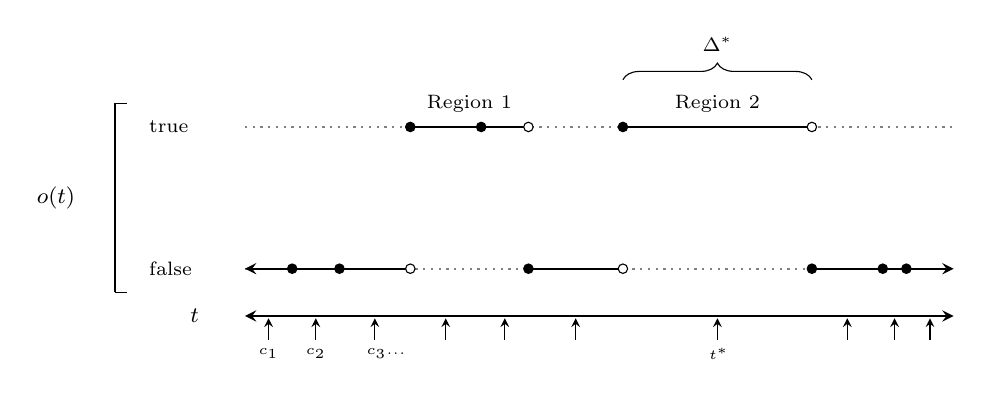
\begin{tikzpicture}[
    axis/.style={thick,<->,>=stealth},
    guide/.style={thick,dotted,gray},
    graphline/.style={thick,black},
    threshmark/.style={thin,->,>=stealth}]

  \def\f{*0.6}

  \draw[axis]
    (1\f,2\f) -- (16\f,2\f);

  \draw[guide]
    (1\f,3\f) -- (16\f,3\f)
    (1\f,6\f) -- (16\f,6\f);

  \draw[graphline,<-,>=stealth]
    (1\f,3\f) -- (4.5\f,3\f);
  \draw[graphline,->,>=stealth]
    (13\f,3\f) -- (16\f,3\f);
  \draw[graphline]
    (4.5\f,6\f) -- (7\f,6\f)
    (7\f,3\f) -- (9\f,3\f)
    (9\f,6\f) -- (13\f,6\f);

  \filldraw[black,draw=black] (2\f,3\f) circle [radius=0.1\f];
  \filldraw[black,draw=black] (3\f,3\f) circle [radius=0.1\f];
  \filldraw[black,draw=black] (4.5\f,6\f) circle [radius=0.1\f];
  \filldraw[black,draw=black] (6\f,6\f) circle [radius=0.1\f];
  \filldraw[black,draw=black] (7\f,3\f) circle [radius=0.1\f];
  \filldraw[black,draw=black] (9\f,6\f) circle [radius=0.1\f];
  \filldraw[black,draw=black] (13\f,3\f) circle [radius=0.1\f];
  \filldraw[black,draw=black] (14.5\f,3\f) circle [radius=0.1\f];
  \filldraw[black,draw=black] (15\f,3\f) circle [radius=0.1\f];
  \filldraw[white,draw=black] (4.5\f,3\f) circle [radius=0.1\f];
  \filldraw[white,draw=black] (7\f,6\f) circle [radius=0.1\f];
  \filldraw[white,draw=black] (9\f,3\f) circle [radius=0.1\f];
  \filldraw[white,draw=black] (13\f,6\f) circle [radius=0.1\f];

%  \draw[threshmark] (1.5\f,3.5\f) -- (1.5\f,3.05\f);
%  \draw[threshmark] (2.5\f,3.5\f) -- (2.5\f,3.05\f);
%  \draw[threshmark] (3.75\f,3.5\f) -- (3.75\f,3.05\f);
%  \draw[threshmark] (5.25\f,6.5\f) -- (5.25\f,6.05\f);
%  \draw[threshmark] (6.5\f,6.5\f) -- (6.5\f,6.05\f);
%  \draw[threshmark] (8\f,3.5\f) -- (8\f,3.05\f);
%  \draw[threshmark] (11\f,6.5\f) -- (11\f,6.05\f);
%  \draw[threshmark] (13.75\f,3.5\f) -- (13.75\f,3.05\f);
%  \draw[threshmark] (14.75\f,3.5\f) -- (14.75\f,3.05\f);
%  \draw[threshmark] (15.5\f,3.5\f) -- (15.5\f,3.05\f);
  
%  \node[align=left] at (1.5\f,3.8\f) {\tiny $o_1$};
%  \node[align=left] at (2.5\f,3.8\f) {\tiny $o_2$};
%  \node[align=left] at (3.75\f,3.8\f) {\tiny $o_3$};
%  \node[align=left,text width=10\f] at (5.25\f,6.8\f) {\tiny $o_4...$};

  \draw[threshmark] (1.5\f,1.5\f) -- (1.5\f,1.95\f);
  \draw[threshmark] (2.5\f,1.5\f) -- (2.5\f,1.95\f);
  \draw[threshmark] (3.75\f,1.5\f) -- (3.75\f,1.95\f);
  \draw[threshmark] (5.25\f,1.5\f) -- (5.25\f,1.95\f);
  \draw[threshmark] (6.5\f,1.5\f) -- (6.5\f,1.95\f);
  \draw[threshmark] (8\f,1.5\f) -- (8\f,1.95\f);
  \draw[threshmark] (11\f,1.5\f) -- (11\f,1.95\f);
  \draw[threshmark] (13.75\f,1.5\f) -- (13.75\f,1.95\f);
  \draw[threshmark] (14.75\f,1.5\f) -- (14.75\f,1.95\f);
  \draw[threshmark] (15.5\f,1.5\f) -- (15.5\f,1.95\f);

  \node[align=left] at (1.5\f,1.2\f) {\tiny $c_1$};
  \node[align=left] at (2.5\f,1.2\f) {\tiny $c_2$};
  \node[align=left,text width=10\f] at (3.75\f,1.2\f) {\tiny $c_3...$};
%  \node[align=left] at (3.75\f,1.2\f) {\tiny $c_3$};
%  \node[align=left,text width=10\f] at (5.25\f,1.2\f) {\tiny $c_4...$};
  \node[align=left,text width=10\f] at (11\f,1.2\f) {\tiny $t^*$};

  \node[align=right,text width=30\f] at (-0.5\f,2\f) {\footnotesize $t$};
  \node[align=left,text width=30\f] at (-0.5\f,3\f) {\scriptsize false};
  \node[align=left,text width=30\f] at (-0.5\f,6\f) {\scriptsize true};

  \draw 
    (-1.5\f,2.5\f) -- (-1.75\f,2.5\f)
    (-1.75\f,2.5\f) -- (-1.75\f,6.5\f)
    (-1.5\f,6.5\f) -- (-1.75\f,6.5\f);

  \node at (-3\f,4.5\f) {\footnotesize $o(t)$};

%  \draw[decorate,decoration={brace,amplitude=10\f},rotate=0] (4.5\f,7\f) -- (7\f,7\f);
  \draw[decorate,decoration={brace,amplitude=10\f},rotate=0] (9\f,7\f) -- (13\f,7\f);

  \node[align=center] at (5.75\f,6.5\f) {\scriptsize Region 1};
  \node[align=center] at (11\f,6.5\f) {\scriptsize Region 2};
  \node[align=center] at (11\f,7.75\f) {\scriptsize $\Delta^*$};
\end{tikzpicture}
\caption[Operation of the BestInterval algorithm]{Operation of the BestInterval algorithm.  Example values of a binary objective function $o(t)$ are shown for a range of input thresholds $t$.  At discrete points defined by observed data values (shown as dots), this objective function can transition, as an observed data point changes its value relative to $t$, and therefore its assigned class.  Two regions in which $o(t) = \mathrm{true}$ are shown.  BestInterval locates all such regions, selects the one with largest measure on $t$ (margin), and returns its centre and margin as $(t^*, \Delta^*)$.  In this example, the centre and margin of region 2 would be returned.  To ensure that $o(t)$ is sampled at sufficient density, candidate thresholds $c_1, c_2, \dots$ are defined between all consecutive values, and beyond the extrema, of $x$; these are indicated by small arrows.  Each $c_i$ is associated with an $o_i$, as $o_i = o(c_i)$.}
\label{fig:mess-bestinterval}
\end{figure}


\begin{figure}[!htbp]
\centering
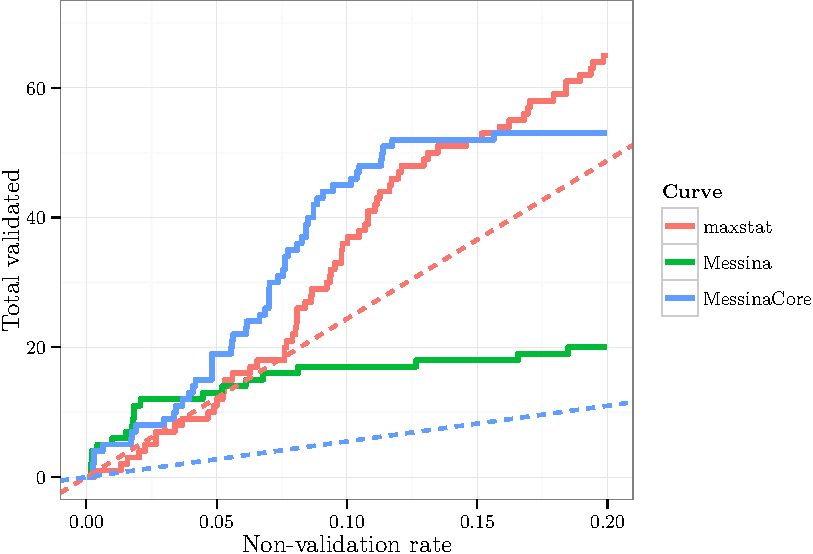
\includegraphics[width=.7\linewidth]{analysis/messina/figure/07-E3-E3-val-detcurves-1}
\caption[]{}\label{fig:mess-val-detabs}
\end{figure}

\begin{figure}[!htbp]
\centering
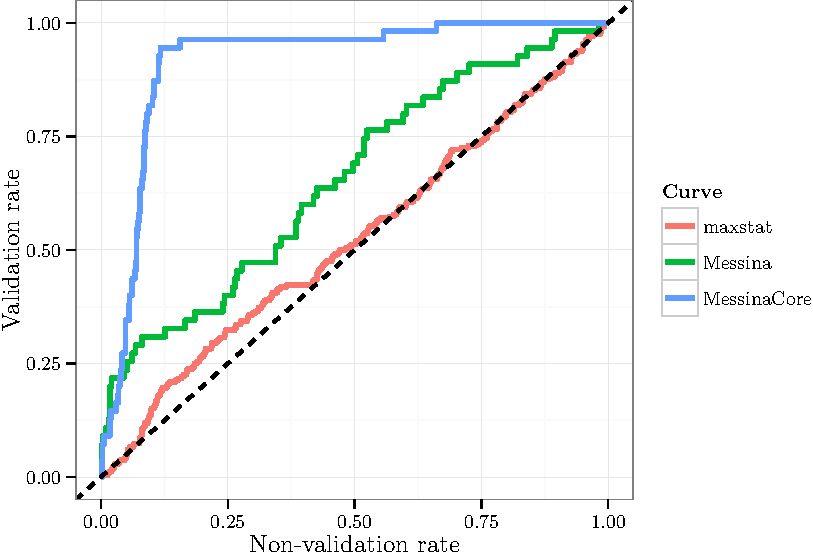
\includegraphics[width=.7\linewidth]{analysis/messina/figure/07-E3-E3-val-detcurves-2}
\caption[]{}\label{fig:mess-val-detrel}
\end{figure}


\end{document}
